\RequirePackage{luatex85}
\documentclass[paper=a4,fontsize=10.5pt]{jlreq}
\usepackage{amsmath,amsfonts,amssymb,mathtools,ascmac,bm,fancybox,calc,multicol,physics,array}
\usepackage[top=20truemm,bottom=20truemm,left=15truemm,right=15truemm]{geometry}
\usepackage{graphicx,color}
\usepackage{tikz,listings,wrapfig,float,xcolor}
\usepackage{url,subcaption,multirow,framed,comment}
\usepackage[unicode,hidelinks,pdfusetitle]{hyperref}
\usepackage{luatexja-fontspec,lltjext}
\usepackage{TeachersGuide}
\hypersetup{
    colorlinks=true,
    citecolor=black,
    linkcolor=black,
    urlcolor=blue
}
\renewcommand{\lstlistingname}{src.}
\newcommand{\srcref}[1]{src.\ \ref{#1}}
\AtBeginDocument{
    \renewcommand{\thelstlisting}{\arabic{lstlisting}}
}

\lstset{
        %プログラム言語(複数の言語に対応,C,C++も可)
    language =TeX,
        %背景色と透過度
    %backgroundcolor={\color[gray]{.90}},
        %枠外に行った時の自動改行
    breaklines = true,
        %自動改行後のインデント量(デフォルトでは20[pt])
    breakindent = 10pt,
        %標準の書体
    basicstyle = \ttfamily\small,
        %コメントの書体
    commentstyle = {\ttfamily \color[cmyk]{1,0.4,1,0}},
        %関数名等の色の設定
    classoffset = 0,
        %キーワード(int, ifなど)の書体
    keywordstyle = {\bfseries \color[cmyk]{1,1,1,1}},
        %表示する文字の書体
    stringstyle = {\ttfamily \color[rgb]{0,0,1}},
        %枠 tは上に線を記載, Tは上に二重線を記載
        %他オプション:leftline,topline,bottomline,lines,single,shadowbox
    frame = leftline,
        %frameまでの間隔(行番号とプログラムの間)
    framesep = 5pt,
        %行番号の位置
    % numbers = left,
        %行番号の間隔
    stepnumber = 1,
        %行番号の書体
    numberstyle = \small,
        %タブの大きさ
    tabsize = 4,
        %キャプションの場所(tbならば上下両方に記載)
    captionpos = t
}
    \usetikzlibrary{intersections,calc,arrows.meta,backgrounds,shapes.geometric,shapes.misc,positioning,fit,graphs,arrows}
    \setlength{\columnsep}{5mm}

    \columnseprule=0.1mm
    \ltjsetparameter{jacharrange={-2}} %日本語以外を欧文扱い

    \renewcommand{\thefootnote}{*\arabic{footnote}}
    \renewcommand{\figurename}{Fig\ }
    \renewcommand{\tablename}{Tbl}
    \newcommand{\figref}[1]{Fig\ \ref{#1}}
    \newcommand{\tabref}[1]{Tbl\ \ref{#1}}

\makeatletter
    \renewcommand{\thefigure}{%
    \thesection.\arabic{figure}}
    \@addtoreset{figure}{section}

    \renewcommand{\thetable}{%
    \thesection.\arabic{table}}
    \@addtoreset{table}{section}

    \@addtoreset{lstlisting}{section}
\makeatother


\title{\textbf{学習指導案}\\ \LaTeXe スタイルファイル 仕様書}
\author{MIZOGUCHI Koki\thanks{Kochi Univeristy of Technology}}
\date{\today}


\begin{document}
\maketitle
\begin{leftbar}
    \section*{ファイル情報}
\end{leftbar}
\begin{framed}
    \begin{multicols}{2}
        \noindent\textbf{スタイルファイル名}\\
        \hspace{0.5em}\verb|TeachersGuide.sty|\\
        \textbf{制作者}\\
        \hspace{0.5em}溝口洸熙\\
        \newline
        \textbf{LICENSE}\\
        \hspace{0.5em}\verb|MIT License|\\
        \textbf{更新・問題}\\
        \hspace{0.5em}{\scriptsize\href{https://github.com/MIZOGUCHIKoki/LaTeX-StyleFile}{https://github.com/MIZOGUCHIKoki/LaTeX-StyleFile}}
    \end{multicols}
\end{framed}
\begin{leftbar}
    \section*{コマンド定義}
\end{leftbar}
\begin{table}[h]
    \begin{tabular}{ll|ll}
        \verb|\tptwidth|      & \verb|tpf|\ 列の幅設定      & \verb|tpt| & 指導案表の1列目のヘッダ文字列 \\
        \verb|\tpswidth|      & \verb|tps|\ 列の幅設定      & \verb|tps| & 指導案表の2列目のヘッダ文字列 \\
        \verb|\tptwidth|      & \verb|tpt|\ 列の幅設定      & \verb|tpt| & 指導案表の3列目のヘッダ文字列 \\
        \verb|\GuidlineTitle| & \textbf{学習指導案}\ と入力
    \end{tabular}
\end{table}
\noindent\ovalbox{\large \verb|\showTitle|}\par
タイトル・指導教員名・指導科目名を印字する.第一引数に指導教員名,第二引数に指導科目名を渡す.\\
\underline{\textbf{入力例}}\\
\verb|\showTitle{(指導教員名)}{(指導科目名)}|\\
\noindent\underline{\textbf{出力例}}
\begin{framed}
    \showTitle{(指導教員名)}{(指導科目名)}
\end{framed}
\begin{leftbar}
    \section*{環境定義}
\end{leftbar}
\noindent\ovalbox{\large\verb|attainmentTarget|}\par
\textbf{到達目標}を記述する.「到達目標」は\\
\noindent\ovalbox{\large\verb|TeachingProcedures|}\par
指導案表の枠を設計する.この環境は\verb|longtable|環境を用いて構築している.従って\verb|tabular|環境同様,列の区切りは\verb| & |を用い,行の区切りは,\verb|\\ |で行う.\par
ヘッダの部分\footnote{デフォルトでは,活動・指導内容・指導上の留意点及び評価}は,それぞれ括弧内のコマンド\footnote{tpf,tps,tpt}で定義しているので,変更したい場合は,適宜\verb| \renewcommand |\footnote{「活動」を「活動内容」に変更したい場合は,{\ttfamily\textbackslash renewcommand\{\textbackslash tpf\}\{活動内容\}}}で更新する.\vspace{0.5em}\\
\ovalbox{\large\verb|tpfcol,tpscol,tptcol|}\par
\verb|tpf, tps, tpt|の列に対して,\verb|tpfcol,tpscol,tptcol|の環境下で編集を行う.これらは,\verb|minipage|環境を用いて構築している.\par
\renewcommand{\tpf}{活動(tpf)}
\renewcommand{\tps}{指導内容(tps)}
\renewcommand{\tpt}{指導上の留意点及び評価(tpt)}
\begin{TeachingProcedures}
    \begin{tpfcol}
        \begin{verbatim}
\begin{tpfcol}
                    
\end{tpfcol} &
            \end{verbatim}
    \end{tpfcol}&
    \begin{tpscol}
        \begin{verbatim}
\begin{tpscol}
        
\end{tpscol} &
        \end{verbatim}
    \end{tpscol}&
    \begin{tptcol}
        \begin{verbatim}
\begin{tptcol}
    
\end{tptcol} \\
        \end{verbatim}
    \end{tptcol}\\
    \hline
\end{TeachingProcedures}
\newpage
\begin{leftbar}
    \section*{作成例}
\end{leftbar}

\renewcommand{\tpf}{活動}
\renewcommand{\tps}{指導内容}
\renewcommand{\tpt}{指導上の留意点及び評価}
\begin{oframed}
    \showTitle{溝口洸熙}{数学}
    \classInfo{1限目}{3年A組}
    \begin{attainmentTarget}
        \(x\)軸方向への平行移動するグラフの関数を推測し,二次関数\(y=a(x-p)^2\)のグラフを描く.
    \end{attainmentTarget}
    \begin{TeachingProcedures}
        \begin{tpfcol}
            \textbf{導入}\\
            前回の事前の学習の確認
        \end{tpfcol} &
        \begin{tpscol}
            \fbox{復習}\\
            二次関数\(y=2x^2-2\)のグラフを描き
            頂点の座標と軸の方程式を求めよ.
        \end{tpscol} &
        \begin{tptcol}
            前時の評価を基に不十分な生徒に机間指導の際に個別に指導する.
        \end{tptcol}\\
        \hline
        \begin{tpfcol}
            \textbf{展開}\\
            グラフから関数の 式 \(y=a(x-p)^2\) を推測 する.
        \end{tpfcol} &
        \begin{tpscol}
            \begin{framed}
                \textbf{課題1}\\
                二次関数\(y=2x^2\)のグラフを\(x\)軸方向に1だけ平行移動したグラフを描く.
            \end{framed}
            \begin{center}
                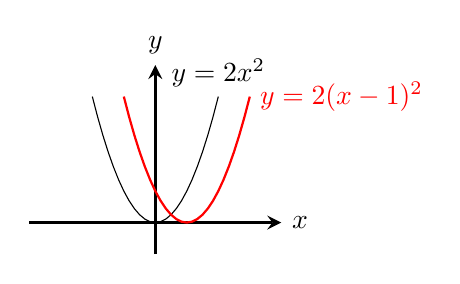
\begin{tikzpicture}[scale=0.4]%倍率
                    \draw[very thick, -stealth] (-4,0)--(4,0) node[right] {$x$};%x軸
                    \draw[very thick, -stealth] (0,-1)--(0,5) node[above] {$y$};%y軸
                    \draw[domain=-2:2] plot(\x, {pow(\x,2)})node[above]{\(y=2x^2\)};
                    \draw[red,domain=-1:3,thick] plot(\x, {pow(\x,2)-2*\x+1})node[right]{\textcolor{red}{\(y=2(x-1)^2\)}};
                \end{tikzpicture}
            \end{center}
        \end{tpscol} &
        \begin{tptcol}
            グラフをかくことで,\(x\)軸方向に1だけ平行移動するとはどういうことかを考えさせる.
        \end{tptcol}\\
    \end{TeachingProcedures}
\end{oframed}
\end{document}